%\documentclass[MTRX3700report.tex]{subfiles}
\documentclass[11pt,a4paper]{article}
% Dpak
% HARDWARE DESIGN
\usepackage{color}
\usepackage{floatrow}
\usepackage{graphics}
% Table float box with bottom caption, box width adjusted to content
\newfloatcommand{capbtabbox}{table}[][\FBwidth]

\begin{document}
  \textcolor{red}
  {
  \textit{Give a detailed description of the design of hardware. The description should include mechanical drawings, location diagrams, electrical circuit schematics, circuit simulation or test results, PCB overlays, wiring diagrams, connector pinout lists, pneumatic/hydraulic circuit diagrams}
  }
  \\The project includes a wide array of hardware types, each with specific requirements to be interfaced with in software and with other the other hardware components. This section will seek to outline the requirements of the individual components used, as well as the scheme with which they were interfaced with each other.

  \subsection{Scope of the Jousting Robot's System Hardware}
    The jousting robot, being composed of 2 interacting systems, namely the Commander and Mobile Robot, has a hardware requirement that was also split into two.
    The Commander hardware and Mobile Robot hardware will be here discussed separately to highlight the differences.

  \subsection{Mobile Robot Hardware Design}
    \subsubsection{Power Supply}
      The Mobile Robot was powered by a Zippy Flightmax 4.2 Ahr Lithium Iron Phosphate (LiFePO4) battery. It consists of 4 series connected cells together producting a typical voltage of 12.8V. The battery is rated for a continuous discharge rate of 126A and a charge rate of 8.4A. The battery is connected to a power supply circuit that has several functions:
      \begin{enumerate}
        \item It provides a connection point for the 12.8V battery.
        \item It provides a connection point for external power supplies if the battery is removed.
        \item It provides 5V DC power at 1.5A to other hardware on the Mobile Robot.
        \item It provides a switch for turning power to the Mobile Robot off or on.
        \item It carries the Pololu 707 Dual VNH3SP30 Motor Driver board and provides power to it.
        \item It provides connection points for motor driver signals, motor leads and encoder signals.
      \end{enumerate}
      \textcolor{red}
      {
      \textit{\textbf{INSERT SCHEMATIC HERE}}
      }
    \subsubsection{Computer Design}
    Description of computer hardware, including all interface circuitry to sensors, actuators, and I/O hardware.
    \subsubsection{Sensor Hardware}

      \begin{itemize}
        \item IR sensors:{ 3 Sharp GP2Y0A41SK0F Infrared Sensors were used to measure distance, with an effective range of 4-40cm, which corresponds to an output voltage of 0.4 to 3.1V. Exceeding 40cm, IR sensor output is saturated. There are 3 connections for the IR sensor,Vcc(nominally 5V), Gnd, and an analog output.}
        \item encoder:{ The rear motor shaft is fitted with a magnetic encoder that provides TTL compatible quadrature signals with a resolution of 64 counts per revolution. The power supply for the encoder is 5V DC and it generates TTL quadrature signals A and B.}
        \item Xbee : {The mobile robot is provided with a Digi International Inc. XBee RF Module with the effective range up to 10m and limited to 250kb/s. The functions of Xbee look like a sensor in robot since it 'sense' the signal from the commander.}
      \end{itemize}
    \subsubsection{Actuator Hardware}
      The primary actuators on the Mobile Robot were the two motors connected to the wheels. The two motors could be  controlled independently allowing for turning functionality. The motor output shafts were connected to multistage planetary gearboxes having reduction ratios of 131.25:1.
      Table \ref{gearmotor} lists the acronyms and abbreviations used in this document.
      \begin{figure}[h]
        \begin{minipage}[b]{0.50\linewidth}
          \raggedleft
          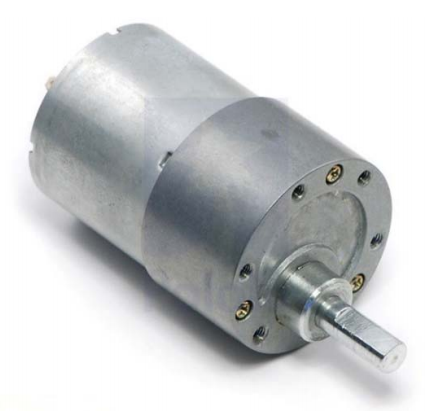
\includegraphics{gearmotor.png}
        \end{minipage}
        \begin{minipage}[b]{0.30\linewidth}

          \begin{tabular}[b]{|l|l|}

            \hline \textbf{Parameter} & \textbf{Value} \\
            \hline Part number & Pololu 1447\\
            \hline No-load speed @ 12 V & 80 RPM\\
            \hline No-load current @ 12 V & 300 mA\\
            \hline Stall current @ 12 V & 5 A\\
            \hline Stall torque @ 12 V & 1.765 Nm\\
            \hline Positive terminal lead & Red\\
            \hline Negative terminal lead & Black\\
            \hline
          \end{tabular}
        \end{minipage}
        \caption{DC gearmotor and specifications specifications}
        \label{gearmotor}
      \end{figure}
      The output shaft from the gearbox was connected to the 90mm wheel via 2 M3 screws that bore down on the shaft flat face.
    \subsubsection{Operator Input Hardware}

    Mobile Robot Hardware Design
  The operator input hardware in the mobil robot is the Xbee and IR sensor. Xbee receive excutives from the commander, hence it is the input hardware. IR sensor detect the distance from the obstacles and input analog signal to the mobile robot.\\
    The operator input hardware in the mobil robot is the Xbee and IR sensor. Xbee receive excutives from the commander, hence it is the input hardware. IR sensor detect the distance from the obstacles and input analog signal to the mobile 
robot.  

    \subsubsection{Operator Output Hardware}
    The output of the mobile robot are PWM motor and Xbee, PWM motor cause the movement of the robot. Xbee can also see as the output hardware since it transmit the robot status back to the commander. Hence it is both input and output hardware.
    \subsubsection{Hardware Quality Assurance}
    The IR sensor is sensitive and it might cause error and unstable value if the system only take 1 IR sensor output value. In order to stablize the IR output data, we store the IR value into an array, and the IR output data is store into the array and it keep overwrite it. In software module, taking the average value in the array and send it to the commander via Xbee will improve the quality of the IR data. The array size is 10 so it have enough buffer to smooth the raw IR data.\\

    Describe any measures that were taken to control (improve) hardware quality and reliability – Heartbeats, brownout conditioning/resets, reset conditions, testing and validation, etc.
  \subsection{Commander Hardware Design}
    \subsubsection{Power Supply}
      Unlike the Mobile Robot, the power requirements of the Commander could be fulfilled from a single 9v battery plugged into the PIC, and all power for peripheral components supplied by the PIC. Due to the many components connected to the power lines, a power rerouting circuit needed to be constructed. This circuit is shown in the next section as it involved interfacing with the PIC.
    \subsubsection{Computer Design}
      Description of computer hardware, including all interface circuitry to sensors, actuators, and I/O hardware.
    \subsubsection{Sensor Hardware}
    \subsubsection{Actuator Hardware}
      There was no actuating hardware present on the Commander, however, the Xbee hardware served as a means of communication between Commander and Mobile Robot.
    \subsubsection{Operator Input Hardware}
      Input hardware consisted of a 2 axis joystick, which is 2 potentiometers at mounted right angles to each other. This joystick also contains a button that can be used by depressing the joystick. A second, separate button was used on the commander for starting and stopping the mobile robot. The commander also included a master power switch.
    \subsubsection{Operator Output Hardware}
      The main output hardware consisted of an LCD screen which displayed the state of the system, as well as basic information about the Mobile Robot to to the operator. 3 LEDs were also in the original design, a power indicator, a radio link integrity indicator, and an LED to indicate the Mobile Robot was in Autonomous mode, however these LED indicators were not implemented in the final product.
    \subsubsection{Hardware Quality Assurance}
      The main hardware quality assurance policy was implemented on the PIC, with a brownout detector enabled by default on the microcontroller.\\

  \subsection{Hardware Validation}
  Details of any systematic testing to ensure that the hardware actually functions as intended.
    \subsubsection{Commander}
    Testing the commander by using LCD display first to make sure the desired outputs are correct, then send the outputs via xbee to verify if the outputs are still correct. \\
    Joystick should systematic testing with the mobile robot first, then connect it to the commander\\
    \subsubsection{Mobile Robot}
    Before attaching the IR sensor into the minimal board, connect it to the demo board fist and test its output analog  voltage whether it match the desire output. Once it was done, combine the IR sensor module and Xbee module, send the IR data via xbee and verify if the IR data are correct after it transmits via xbee.\\
    In order to test the PWM motor if it actually functions as intended, attach the joystick direct to the robot minimal board, it can isolate the serial module and test the PWM motor hardware only. \\

  \subsection{Hardware Calibration Procedures}
    Procedures for calibration required in the factory, or in the field.
    \subsubsection{Commander}
    \subsubsection{Mobile Robot}
    Calibration of Xbee module are more like 'enable / disable the function 'of Xbee. They need to be disable after the data transmission are finish. 

  \subsection{Hardware Maintenance and Adjustment}
    Routine adjustment and maintenance procedures.
    \subsubsection{Commander}
    \subsubsection{Mobile Robot}


\end{document}
